\documentclass{article}

\usepackage{geometry}
\usepackage{amsmath}
\usepackage{graphicx}
\usepackage{listings}
\usepackage{hyperref}
\usepackage{multicol}
\usepackage{fancyhdr}
\pagestyle{fancy}
\hypersetup{ colorlinks=true, linkcolor=black, filecolor=magenta, urlcolor=cyan}
\geometry{ a4paper, total={170mm,257mm}, top=20mm, right=20mm, bottom=20mm, left=20mm}
\setlength{\parindent}{0pt}
\setlength{\parskip}{1em}
\renewcommand{\headrulewidth}{0pt}
\lhead{Competitive Programming - Arkavidia V}
\fancyfoot[CE,CO]{\thepage}
\lstset{
    basicstyle=\ttfamily\small,
    columns=fixed,
    extendedchars=true,
    breaklines=true,
    tabsize=2,
    prebreak=\raisebox{0ex}[0ex][0ex]{\ensuremath{\hookleftarrow}},
    frame=none,
    showtabs=false,
    showspaces=false,
    showstringspaces=false,
    prebreak={},
    keywordstyle=\color[rgb]{0.627,0.126,0.941},
    commentstyle=\color[rgb]{0.133,0.545,0.133},
    stringstyle=\color[rgb]{01,0,0},
    captionpos=t,
    escapeinside={(\%}{\%)}
}

\begin{document}

\begin{center}
    \section*{Langkah Catur Mirip Kuda} % ganti judul soal

    \begin{tabular}{ | c c | }
        \hline
        Batas Waktu  & 1s \\    % jangan lupa ganti time limit
        Batas Memori & 512MB \\  % jangan lupa ganti memory limit
        \hline
    \end{tabular}
\end{center}

\subsection*{Deskripsi}

Arvi sedang memainkan permainan yang baru saja dia buat, dinamakan loncat kuda. 
Aturannya sederhana, sebuah kuda catur harus digerakkan menuju sebuah titik akhir pada papan catur $M \times N$
Pada permainan ini, kuda dapat meloncat sejauh $A$ langkah kedepan dan $B$ langkah kesamping. 
(Tidak harus 2 langkah kedepan dan 1 langkah kesamping seperti kuda catur biasa)
Selain itu, terdapat sejumlah jebakan pada papan catur yang tidak boleh diinjak kuda.

Berikut adalah contoh konfigurasi papan.

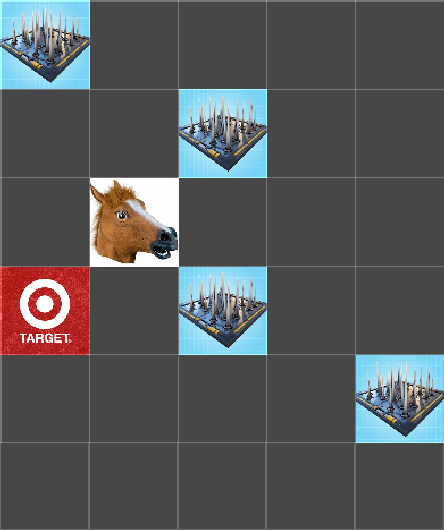
\includegraphics[width=100px]{Initial-Configuration}

Misi Anda adalah membantu Arvi agar dapat menyelesaikan sebuah konfigurasi papan dalam langkah terkecil.
Misalnya, untuk $(A,B)=(3,1)$,konfigurasi diatas dapat diselesaikan dalam langkah-langkah berikut.

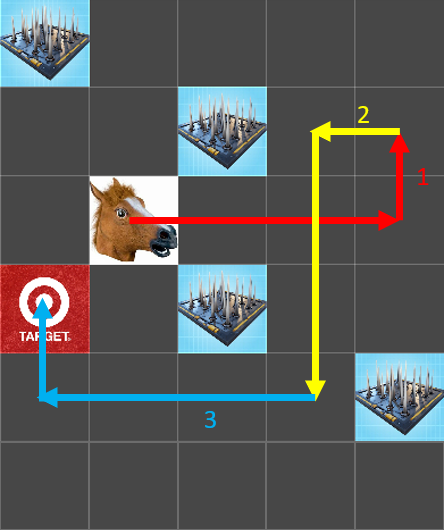
\includegraphics[width=100px]{Movelist}

\subsection*{Format Masukan}

Baris pertama terdiri dari dua bilangan positif $M$ dan $N$ ($1 \leq M \leq 100.000$, $1 \leq N \leq 100.000$) yang menyatakan besar papan.
$N$ baris selanjutnya diisi dengan $M$ karakter yang merupakan salah satu dari: X, -, K, O.

\begin{itemize}
    \setlength\itemsep{0pt}
    \item Karakter X merupakan sebuah perangkap pada petak tersebut,
    \item Karakter - berarti petak tidak ditempati hal apapun,
    \item Karakter K menunjukkan adanya kuda pada petak tersebut, dan
    \item Karakter O adalah titik tujuan kuda catur.
\end{itemize}

Baris terakhir teridiri dari 2 bilangan positif $A$ dan $B$ ($1 \leq A \leq 100.000$, $1 \leq B \leq 100.000$) yang merupakan besar loncatan kuda.

\subsection*{Format Keluaran}

Untuk setiap kasus uji, tuliskan jumlah langkah minimum yang harus dilakukan agar kuda dapat mencapai titik tujuannya.
\\

\begin{multicols}{2}
\subsection*{Contoh Masukan}
\begin{lstlisting}
5 6
X - - - -
- - X - -
- K - - -
O - X - -
- - - - X
- - - - -
3 1
\end{lstlisting}
\columnbreak
\subsection*{Contoh Keluaran}
\begin{lstlisting}
3
\end{lstlisting}
\vfill
\null
\end{multicols}

% \subsection*{Penjelasan}
% Jika dibutuhkan, tambahkan penjelasan di sini

\pagebreak

\end{document}

